\documentclass[twocolumn]{aastex631}

% Packages
\usepackage{microtype}  % ALWAYS!
\usepackage{amsmath}
\usepackage{amsfonts}
\usepackage{amssymb}
\usepackage{multirow}
\usepackage{tikz}
\usepackage{xcolor}
\usepackage{soul}

\definecolor{pink}{RGB}{232,132,161}
\definecolor{yellow}{RGB}{255,213,0}

\newcommand{\kc}[1]{\textcolor{yellow}{\textbf{kc: #1}} }
\newcommand\shadetext[2][]{%
  \setbox0=\hbox{{\special{pdf:literal 7 Tr }#2}}%
  \tikz[baseline=0]\path [#1] \pgfextra{\rlap{\copy0}} (0,-\dp0) rectangle (\wd0,\ht0);% 
  }
\newcommand{\gb}[1]{\shadetext[left color=blue, right color=red, middle color=lime, shading angle=45]{\textbf{g: #1}} }
% \newcommand{\ecite}[1]{\textcolor{pink}{\textbf{: #1}} }
% \newcommand{\e}[1]{\textcolor{yellow}{\textbf{: #1}} }

\newcommand{\remove}[1]{\textcolor{red}{#1}}
\newcommand{\add}[1]{\textcolor{green}{#1}}

\newcommand{\mlg}{\ensuremath{M_{\rm LG}}}
\newcommand{\mmto}{\ensuremath{M_{\rm M31}}}
\newcommand{\mmw}{\ensuremath{M_{\rm MW}}}
\newcommand{\vtan}{\ensuremath{v_\textrm{tan}}}
\newcommand{\vrad}{\ensuremath{v_\textrm{rad}}}
\newcommand{\ms}[1]{\ensuremath{M_{*{#1}}}}
\newcommand{\reflabel}[1]{\ensuremath{^{\mbox{\scriptsize{#1}}}}}
\newcommand{\scsep}{\ensuremath{\rm r_{sep}/r_{vir}}}
\newcommand{\scvel}{\ensuremath{\rm v_{rel}/v_{vir}}}
\newcommand{\subcat}{\textit{Subhalo Catalog}}
\newcommand{\starcat}{\textit{Subhalo + Stellar Mass Catalog}}
\newcommand{\paircat}{\textit{Full Pair Catalog}}
\newcommand{\Rvir}{\ensuremath{\rm R_{vir}}}

% Style tweaks
% \renewcommand{\twocolumngrid}{\onecolumngrid}
% \setlength{\parindent}{1.1\baselineskip}
% \sloppy\sloppypar\raggedbottom\frenchspacing

%%%%%%%%%%%%%%%%%%%%%%%%%%%%%%%%%%%%%%%%%%%%%%%%%%%%%%%%%%%%%%%%%%%%%%%%%%%%%%%%
\shorttitle{Frequency of galaxy pairs}
\shortauthors{Chamberlain et al.}

%%%%%%%%%%%%%%%%%%%%%%%%%%%%%%%%%%%%%%%%%%%%%%%%%%%%%%%%%%%%%%%%%%%%%%%%%%%%%%%%
\graphicspath{{./}{../plots/paper1/}}
% Missions
\newcommand{\project}[1]{\textsl{#1}}

% Packages / projects / programming
\newcommand{\package}[1]{\textsl{#1}}
\newcommand{\acronym}[1]{{\small{#1}}}
\newcommand{\github}{\package{GitHub}}
\newcommand{\python}{\package{Python}}
\newcommand{\astropy}{\package{Astropy}}

% Stats / probability
\newcommand{\given}{\,|\,}
\newcommand{\norm}{\mathcal{N}}
\newcommand{\pdf}{\textsl{pdf}}

% Maths
\newcommand{\dd}{\mathrm{d}}
\newcommand{\transpose}[1]{{#1}^{\mathsf{T}}}
\newcommand{\inverse}[1]{{#1}^{-1}}
\newcommand{\argmin}{\operatornamewithlimits{argmin}}
\newcommand{\mean}[1]{\left< #1 \right>}

% Non-scalar variables
\renewcommand{\vec}[1]{\ensuremath{\bs{#1}}}
\newcommand{\mat}[1]{\ensuremath{\mathbf{#1}}}

% Unit shortcuts
\newcommand{\Msun}{\ensuremath{\mathrm{M}_\odot}}
\newcommand{\Mjup}{\ensuremath{\mathrm{M}_{\mathrm{J}}}}
\newcommand{\kms}{\ensuremath{\mathrm{km}~\mathrm{s}^{-1}}}
\newcommand{\pc}{\ensuremath{\mathrm{pc}}}
\newcommand{\kpc}{\ensuremath{\mathrm{kpc}}}
\newcommand{\Mpc}{\ensuremath{\mathrm{Mpc}}}
\newcommand{\kmskpc}{\ensuremath{\mathrm{km}~\mathrm{s}^{-1}~\mathrm{kpc}^{-1}}}
\newcommand{\dayd}{\ensuremath{\mathrm{d}}}
\newcommand{\yr}{\ensuremath{\mathrm{yr}}}
\newcommand{\Myr}{\ensuremath{\mathrm{Myr}}}
\newcommand{\Gyr}{\ensuremath{\mathrm{Gyr}}}
\newcommand{\Kel}{\ensuremath{\mathrm{K}}}
\newcommand{\masyr}{\ensuremath{\mathrm{mas}~\mathrm{yr}^{-1}}}
\newcommand{\muasyr}{\ensuremath{\mu\mathrm{as}~\mathrm{yr}^{-1}}}

% Misc.
\newcommand{\bs}[1]{\boldsymbol{#1}}

% Astronomy
\newcommand{\DM}{{\rm DM}}
\newcommand{\feh}{\ensuremath{{[{\rm Fe}/{\rm H}]}}}
\newcommand{\df}{\acronym{DF}}

% TO DO
\newcommand{\todo}[1]{{\color{red} TODO: #1}}
\newcommand{\apw}[1]{{\color{blue} APW says: #1}}

% Projects
\newcommand{\gaia}{\textsl{Gaia}}
\newcommand{\gaiadr}{\textsl{Gaia}~\acronym{EDR3}}
\newcommand{\hst}{\textsl{HST}}
\newcommand{\ill}{\textsl{Illustris}}
\newcommand{\tng}{\textsl{IllustrisTNG}} 



% Affiliations
\newcommand{\affuofa}{University of Arizona, 933 N. Cherry Ave,
    Tucson, AZ 85721, USA}

%% This is the end of the preamble.  Indicate the beginning of the
%% manuscript itself with \begin{document}.

\begin{document}

\title{
  Frequency of low and high mass galaxy pairs in the IllustrisTNG cosmological simulation
}

\author[0000-0001-8765-8670]{Katie~Chamberlain}
\affiliation{\affuofa}

\author[0000-0003-0715-2173]{Gurtina Besla}
\affiliation{\affuofa}


\begin{abstract}
  
\end{abstract}

%%%%%%%%%%%%%%%%%%%%%%%%%%%%%%%%%%%
\section{Introduction} \label{sec:intro}

\begin{itemize}
    \item Galaxy mergers are a feature of LCDM and support the growth of galaxies across cosmic time.
    \item The frequency of finding pairs tells us about how often we might expect: starbursts, SMBH mergers, the importance/role of mergers in building stellar mass/morphologies of galaxies today, SFHs, etc. 
    \item pair fraction at high masses has been well studied both obs and theoretically. There are studies of high mass (Mstar = 5e9-1e11Msun) pairs. These studies are typically done in projection for comparison to observational campaigns.
    \item There are studies of low mass pairs (define what you mean by this), but only at low z, or as satellites of more massive systems (analogs of LG). 
    \item in the era of jwst, these studies will be pushed to lower masses and high z, however, from a theory perspective, pair fractions at low masses have been under-studied (first 2 ish paragraphs ~ )
    \item There are reasons to believe that high and low mass (Mstar = 1e8-5e9Msun) pairs might evolve differently, so it's important to study the low mass end too. 

    \item Also, major and minor mergers are important for different reasons, so studying them as separate systems is well motivated.
        - is major high mass vs major low mass different, etc since these two types of mass ratios lead to different things 
        - importance of mergers in high vs low mass galaxies (major mergers may be less important to SFH of Universe etc - look at sabrina's papers)
    \item Systematically understanding the underlying difference between low and high mass pairs, Projected vs. 3D separations/pairs Two routes of studying galaxy pairs are through observations and simulations, but simulations allow us to fully understand the 3D position and velocity of objects. 
    \item in this study, we'll be quantifying the pair fraction of low mass pairs, and self consistently comparing to the pair fraction of high mass systems
    \item In this work, we aim to characterize the pair fraction of both high and low mass galaxies, major and minor pairs, consistently as a function of time. 
\end{itemize}
cite Stierwalt for low mass pairs 4485/4490 (iso vs non iso pairs) 
Pearson Besla 2016 
Pearson Besla 2018 4485/4490
Luber Pearson Besla 
Nevin 

Discussion section: 
what does this mean for our understanding of the LG (isolated mass analogs) 
ngc 4490/4485 as another low z example (minor dwarf pair) 


%%%%%%%%%%%%%%%%%%%%%%%%%%%%%%%%%%%
%%%%%%%%%%%%%%%%%%%%%%%%%%%%%%%%%%%
 \section{Methodology}\label{sec:methods}
We aim to quantify and characterize the frequency, or occurrence rate, of low mass ($\rm\ms{}=10^{8}-5\times 10^{9}\Msun$) and high mass ($\rm\ms{}=5\times10^{9}-10^{11}\Msun$) galaxy pairs in cosmological simulations as a function of cosmic time. 
To this end, we utilize the IllustrisTNG simulation to select halo pairs at each snapshot according to a strict set of selection criteria as outlined in the remainder of this section. 
In Sec.~\ref{sec:methods-sims}, we provide motivation for and details of the simulation utilized in this study.
Sec.~\ref{sec:methods-halos} outlines the initial mass cuts used to define our \subcat, to which we will 
add stellar mass information. %consist of the set of subhalos from which we will select pairs.
Sec.~\ref{sec:methods-am} outlines the abundance matching prescription used to associate dark matter subhalos with stellar masses, and the creation of the \starcat, from which we will select pairs.
Sec.~\ref{sec:methods-pairs} describes the second set of selection criteria that we use to finally construct the \paircat. 
% Finally, Sec.~\ref{sec:pairprops} details some of the properties of our entire pair sample, including the total number of pairs and stellar mass ratios. -- Note: created new section


%%%%%%%%%%%%%%%%%%%%%%%
% Sim details section %
    \subsection{Simulation details} \label{sec:methods-sims}
        % Brief description of TNG hydro and which run we use.
    The \tng\ project~\citep{TNG1, TNG2, TNG3, TNG4, TNG5} consists of a suite of dark-matter-only $N$-body as well as full physics cosmological simulations consistent with the \textit{Planck2015} \lcdm\  cosmology~\citep{Planck2015}.
    In this study we utilize data from the main high resolution, full physics run of the (110.7\Mpc)$^3$ volume simulation, \textsl{TNG100-1}, which follows the evolution of baryons and $1820^3$ dark matter particles from $z=127$ to $z=0$. 

      % subfind, sublink, and groups and subhalos
    We utilize the group catalogs produced by the \texttt{SUBFIND} algorithm~\citep{springel2001,dolag09}. 
    This catalog was created using the Friends-of-Friends (FoF) algorithm~\citep{davis1985}, which links nearby particles to define large halos of associated particles, from which subhalos are identified as over-dense and gravitationally bound dark matter structures.
    In addition, we utilize the merger trees provided by the \texttt{SUBLINK} algorithm~\citep{rg15}, which tracks subhalos between snapshots using their DM particle data in order to trace mass growth and merger histories of subhalos between snapshots.
    
    The high resolution of the TNG100-1 simulation permits a direct comparison of low mass and high mass galaxy pair fractions without concern for incompleteness at the low mass end from unresolved low mass pairs (details in~\ref{sec:methods-halos}).
    Additionally, the volume of this simulation provides a large enough sample of massive halo pairs to allow for a statistically significant comparison. 

    % Baryonic process are known to affect the structure and formation of dark matter halos of low mass ($M_*\lesssim 1\times10^9\Msun$) subhalos in simulations~\citep[see e.g.][and references therein]{Sales:2022}.
    % Additionally, the shallow potential well of dwarf galaxies compared to their massive counterparts may lend themselves more easily to disruption from baryonic processes such as supernova feedback and reionization~\citep{}, resulting in fewer low mass halos ($\lesssim 5\times10^{10}$) in hydrodynamic simulations~\citep{vogelsberger14B}.
% End sim details     %
%%%%%%%%%%%%%%%%%%%%%%%

%%%%%%%%%%%%%%%%%%%%%%%%%%    
% Choosing halos section %
    \subsection{Choosing dwarf and massive subhalos in TNG} \label{sec:methods-halos}
    Galaxies form in dark matter subhalos, so our pair sample will consist of pairs of subhalos within these larger group structures.
    In this section, we've outlined the steps to create the \subcat, which we will utilize to assign stellar masses to each of the dark matter subhalos. 
 
    We are interested in the inherent frequency of galaxy pairs in the field. 
    The largest perturbers of a subhalo are typically part of the same group, as a consequence of the FoF algorithm. 
    Thus, selecting from the most massive subhalos of a group ensures that the pairs are roughly isolated. 
    In addition, we have confirmed that over 99\% of subhalos are isolated from large perturbers within 1 \Mpc.
    This isolation criteria, which is a feature of our selection process, ensures that the final selected pairs are not dynamically influenced by nearby massive groups. 

    The following selection process is repeated for each snapshot of the simulation over a redshift range of $z=0-\sim4$, at which point the population of massive subhalo pairs falls off rapidly (see Sec.~\ref{sec:pairprops} for more details).

    First, at each snapshot, we invoke a cut on the total FoF group mass, \MG{}, given by \texttt{Group\_M\_TopHat200} in the TNG100 group catalogs. 
    We define the group mass range for low mass and high mass groups as 
    \begin{align*}
        \mbox{\textbf{low mass:}}&\,\rm M_{G} = 8\times 10^{10}- 5\times 10^{11}\,\Msun \\ 
        \mbox{\textbf{high mass:}}&\, \rm M_{G}=10^{12}- 6.5\times10^{12}\,\Msun.
    \end{align*}
    The group mass criteria is fixed for all redshifts, which means that some low mass groups at high $z$ may be the progenitors of high mass systems at $z=0$.
    Note that all masses used in this analysis are physical units, such that masses from the group catalogs are divided by $h$ to get units of \Msun. 

    Selecting low mass pairs from the low group mass range ensures that we are not selecting satellite systems in the halos of more massive systems, nor low mass pairs in a large group. 
    Additionally, $z\sim0$ groups of high mass will host isolated mass analogs of the MW--M31 and MW--LMC systems, while the low mass groups will host isolated mass analogs of an LMC--LMC or LMC--SMC pair. 
    
    
        % explain what halos we will move forward with. 
    From the set of groups that pass the group mass cut, we create a catalog of all subhalos within each group that pass a ``current mass" threshold, such that the subhalo mass at the given snapshot, given by \texttt{SubhaloMass} field in the group catalogs, is
    \begin{equation*}
    \mbox{\textbf{min. subhalo mass:}}\,
    \Mhalo > 1\times10^{9}\Msun.\footnote{Note that for the TNG100 hydro run, the subhalo mass is the total sum of all bound dark \textit{and} baryonic matter.}
    \end{equation*}
    This lower mass threshold ensures that our halos are resolved into $>100$ particles, and thus should be robust to the \subfind\ and \sublink\ algorithms, even at the low mass end.  
    For each subhalo that passes both of the above criteria, we use the \sublink\ merger trees to identify the maximum subhalo mass achieved by the subhalo, \Mpeak. 
    We consider only the given snapshot and all previous snapshots in the determination of \Mpeak.
    
    All subhalos in a given snapshot that pass both the group and current mass selection criteria will be added to our full sample of subhalos, which we call the \subcat. 
    The catalog contains subhalos at each snapshot from $z=0-\sim4.2$ (snapshot numbers 20-99) and their associated properties, namely: Subhalo ID, FoF Group Number, current subhalo mass \Mhalo, and peak halo mass \Mpeak.
    From here, we will use further selection criteria to narrow down this large sample and to match pairs of subhalos in each group.
% End choosing halos     %
%%%%%%%%%%%%%%%%%%%%%%%%%%    

%%%%%%%%%%%%%%%%%%%%%%%%%%%%%%    
% Abundance matching section %
    \subsection{Abundance matching} \label{sec:methods-am}
    We will be utilizing a stellar mass to halo mass (SMHM) relationship to assign stellar masses to each of the subhalos in our \subcat.  
    There are a few reasons we opt to assign stellar masses to our subhalos, rather than use those computed by the simulation. 

    Primarily, applying an abundance matching prescription to assign stellar masses to each of the dark matter halos allows us to account for the observed spread in the SMHM relationship. 
    This is particularly important in the low mass regime ($M_h \lesssim 10^{11}\Msun$) where the scatter in the SMHM function is large, $\sim 1$dex at $M_{h}\sim 10^{10}\Msun$. 
    In addition, using stellar masses as calculated from abundance matching allows us to side step any simulation-dependent stellar mass effects.
    In the case of TNG100 specifically, stellar masses of low mass galaxies are often overestimated compared to the galaxy luminosity function at the low mass end\cite{}. 
    Using an observationally-calibrated abundance matching prescription will thus lead to a more robust result for comparison with and predictions for observations. 
    Finally, utilizing an abundance matching prescription allows us to directly compare results between dark matter only and hydro simulations, since the stellar masses are assigned the same way. 
    We make brief note of results for our equivalent analysis using the dark matter only, TNG100-Dark simulation as well in Sec.~\ref{sec:discussion}.\kc{need to specify section once written}
    
        % what am prescription are we using? 
    We use the abundance matching relationship presented in~\citet{Moster2013}, which provides an analytic prescription to assign stellar masses to dark matter halos. 
    The~\citet{Moster2013} relationship is a function of subhalo mass, redshift, and includes terms to account for the systematic scatter in the SMHM relationship, with larger scatter at lower halo masses.
    
        % realizations? 
    We elect to use the maximum subhalo mass \Mpeak\ in the stellar mass calculation, rather than the subhalo mass at the given snapshot.
    We also use the current redshift of the given snapshot, $z_{snap}$, of each subhalo in the stellar mass calculation. 
    Thus, $\ms{}=f(\Mpeak,z_{snap})$. 
    
    Using \Mpeak\ mass allows us to remain robust to scenarios in which a secondary has formed most of its stars, then loses a significant portion of its dark matter content through tidal interactions with a primary, but retains the bulk of its stellar content.
    In fact, \citet{Munshi2021} found that the stellar mass of subhalos at $z=0$ in the ``Marvel-ous Dwarfs" and ``DC Justice League" zoom simulations are more closely correlated with $M_{peak}$ than the $z=0$ halo mass for halos with peak halo mass $10^8<M_{\rm peak}<10^{11} \Msun$. 

    Using $z_{snap}$ means that we allow the stellar mass of both the primary and secondary halo to change as a function of redshift, even after the secondary has entered the primary's halo. %and do not immediately cease star formation. 
    This assumption is consistent with findings from~\cite{Akins2021}, which found that massive dwarf satellites ($M_*\approx 10^8-10^9\, \Msun$) entering MW-mass host halos are rarely quenched, and with~\cite{geha13} which finds that dwarfs $>1\Mpc$ from a MW-type galaxy are often star forming and rarely quenched.
    Additionally, the SAGA survey has found that large satellites of MW-type galaxies are often very blue, with infall into the halo spurring high rates of star formation due to the large gas fraction in dwarfs~\citep{Mao2021}. 
    % maybe need a note here on whether this is fair to extend to higher mass system?

    We then calculate the stellar mass for a given subhalo by gaussian sampling each of the fitting parameters of the analytic framework from~\cite{Moster2013}, in order to account for the spread in the SMHM relationship.
    We generate a single stellar mass ``realization" of the full \subcat\ by calculating a stellar mass for each subhalo, using an independent draw the SMHM distribution for each subhalo. 
    For each snapshot, we repeat this process 1000 times to generate 1000 realizations of stellar masses for the \subcat.
    The resulting catalog is called the \starcat, and consists of the set of all subhalos from the \subcat, as well as the 1000 stellar mass realizations. 
    Each realization is treated as an independent sample of galaxy stellar masses, which will allow us to report realistic spreads of pair properties.

    % As mentioned in a footnote in Sec.~\ref{sec:methods-halos}, the total halo mass of subhalos in the hydro simulation includes the mass of both dark matter and baryonic particles. 
    % In TNG100-1, the DM particle mass is decreased XX\% compared to the DM particle mass in \tng100-1 Dark to account for the additional mass of baryons, such that the total mass of the halo will remain roughly the same between the dark matter only and hydro simulations. 
    % Since the~\citet{Moster2013} AM relation was calibrated using DM subhalos from the \texttt{MilleniumII} dark matter only simulation, we will use the total subhalo mass from the TNG100 hydro simulation as a proxy for the corresponding DM halo mass in the TNG100-1 Dark run, \texttt{SubhaloMass}. 


% End Abundance matching %
%%%%%%%%%%%%%%%%%%%%%%%%%%   

%%%%%%%%%%%%%%%%%%%%%%%%%%    
% Pair selection section %
    \subsection{Pair selection}\label{sec:methods-pairs}
    Starting from the \starcat, here we outline the pair matching process through which we generate the \paircat. 
    At each redshift, and for each stellar mass realization, we will identify subhalo pairs consisting of a "primary" and a "secondary", where primaries are the more massive of the pair by stellar mass.

    % justify why we want to use stellar mass to define things
    %A majority of the literature uses the definition of "major" and "minor" pairs based on the stellar mass of the objects. This is true as well for observational pair samples, such as Lotz 2011, wherein the halo mass of the objects is unknown, and thus the stellar mass is used to define the mass ratio of the pair. In order to reproduce statistics that can be meaningfully compared to observations/can be used to inform observations, we opt to define our pair sample via the stellar masses from the abundance matching prescription given in Sec.~\ref{sec:methods-am}. 

    %%% 
    % begin subsubsection
    \subsubsection{Selecting primaries}
        Primary galaxies (equivalently, ``primary subhalos") are the most massive galaxy of their FoF group by stellar mass, such that each group can have at most one primary galaxy.  
        Each stellar mass realization is treated independently, such that the subhalo identified as the primary of a group may change between stellar mass realizations. 

        At a given snapshot, and for each stellar mass realization, we rank order the subhalos of each group by stellar mass. 
        Primaries must be the most massive subhalo in their group, and pass the following stellar mass criteria:         
        \begin{align*} 
        \mbox{\textbf{low mass primaries:}}&\, 10^{8}< \rm M_{*1} < 5\times10^{9}\Msun \\ 
        \mbox{\textbf{high mass primaries:}}&\, 5\times 10^{9}< \rm M_{*1} < 10^{11}\Msun.
        \end{align*}
        The stellar mass criteria is fixed, and does not change as a function of redshift. 
        At $z=0$, the stellar mass range for low mass primaries corresponds to isolated analogs of the LMC or M33, while the high mass primaries represent isolated analogs of the MW or M31. 

        % The median number of primaries in a single stellar mass realization at $z=0$ is XX dwarf primaries and XX massive primaries (see Sec.~\ref{sec:pairprops} for more info). 
        Since our selection is based on stellar mass, and there is a large spread in the SMHM relation, a primary subhalo may not be the most massive subhalo in terms of total subhalo mass. 

    % end  primary subsubsection
    %%% 
    
    %%% 
    % begin secondary subsubsection
    \subsubsection{Selecting secondary companions}
        As before, the selection of secondary companions occurs independently for each stellar mass realization, and for each snapshot. 
        Secondary subhalos are defined as the second most massive subhalo in a FoF group by stellar mass. 
        Secondary subhalos with stellar mass $M_{*2}$ must have a stellar mass ratio:
        \begin{align*}
            &\mbox{\textbf{stellar mass ratio:}}\,      
            M_{*2}/M_{*1} > 1/10.
        \end{align*} 
        We do not include companions with a stellar mass ratio $M_{*2}/M_{*1} <1/10$ due to the lower bound subhalo mass criteria of $\Mhalo=10^9$, which has at least a the corresponding stellar mass of $10^6\Msun$ at $z=0$.
        The stellar mass ratio criterion ensures completeness of the sample, even at the lowest stellar masses considered.

    \subsubsection{Creating the pair catalog}
        Pairs consist of a single primary and secondary in a FoF group as selected via the criteria above. 
        Each pair is categorized as either a major or minor pair based on the stellar mass ratio between the primary and secondary. 
        The stellar mass ratio criteria for major and minor pairs are:
        \begin{align*} 
        \mbox{\textbf{major pair:}}&\, \frac{1}{4}\leq \frac{\rm M_{*2}}{\rm M_{*1}}< 1 \\ 
        \mbox{\textbf{minor pair:}}&\, \frac{1}{10}\leq \frac{\rm M_{*2}}{\rm M_{*1}} < \frac{1}{4}.
        \end{align*}

        For each pair, we calculate the physical separation (\kpc, not comoving \kpc) between the two subhalos using the \texttt{SubhaloPos} field from the group catalogs, and we require that each pair have a minimum separation of $15 \kpc$ between the primary and secondary.
        The minimum separation cut is 20 times the smoothing length of the simulation at $z=0$ which ensures that \subfind can identify the subhalos as distinct objects. 

        If a primary subhalo does not have a companion that meets the stellar mass ratio criteria and separation criteria, the subhalo will still be considered a primary. 
        We refer to all primaries without companions as ``isolated primaries."
        The total number of primaries includes both isolated primaries and those with companions, and is larger than or equal to the total number of pairs.

        For each snapshot and each of the 1000 realizations of the abundance matching prescription, we create a set of isolated primaries and pairs. 
        The final \paircat is the collection of all isolated primaries and pairs at each snapshot, and includes the following information: for each isolated primary, we store the subhalo mass and stellar mass from the given realization; from each pair we store the primary and secondary subhalo masses, stellar masses, group radius, and separation.
        
    % end secondary subsubsection
    %%%     
% Pair selection end %
%%%%%%%%%%%%%%%%%%%%%%

% Methods end %
%%%%%%%%%%%%%%%
%%%%%%%%%%%%%%%

%%%%%%%%%%%%%%%%%%%%%%%%%
% begin pair prop plots %  
\begin{figure*}[htb]
    \centering
    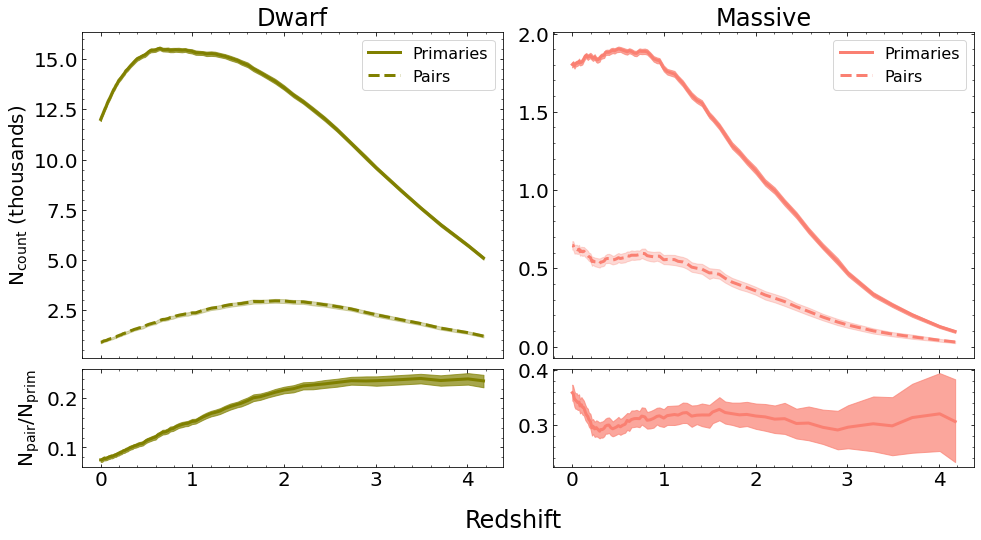
\includegraphics[width=\textwidth]{counts_1000.png}
    \caption{(Top) Number of isolated low mass (left) and high mass (right) primaries and pairs as a function of redshift.
    The solid and dashed lines represent the median of the set of total counts from each of the 1000 stellar mass realizations in the \paircat, while the shaded regions depict the 1-99 percentile spread of the median.
    There are approximately 8 times as many low mass primaries as high mass primaries. 
    % dwarf galaxies
    The low mass primary count (left) peaks at $z=1$ (with $\sim 15000$ primary subhalos per realization), while the low mass pair count peaks at $z=2$ (with $\sim 3000$ pairs per realization). 
    % Massive galaxies (right)
    The high mass primary count (right) peaks at $z\sim1$ (with $\sim 1900$ primary subhalos per realization), while the high mass pair count peaks at $z=0$ (with $\sim 700$ pairs per realization). 
    (Bottom) Total pair fraction (fraction of primaries with a companion secondary) as a function of redshift (see Sec.~\ref{sec:pairprops} for calculation details).
    Low mass pair fraction is approximately flat between $z=2.5-4$, and decreases from $z=2.5$ to $z=0$. 
    The high mass total pair fraction is flat or decreasing from $z=1$ to $z=4$, but spikes sharply between $z=0-0.25$.}
    \label{fig:counts}
\end{figure*}

\begin{figure*}[htb]
    \centering
    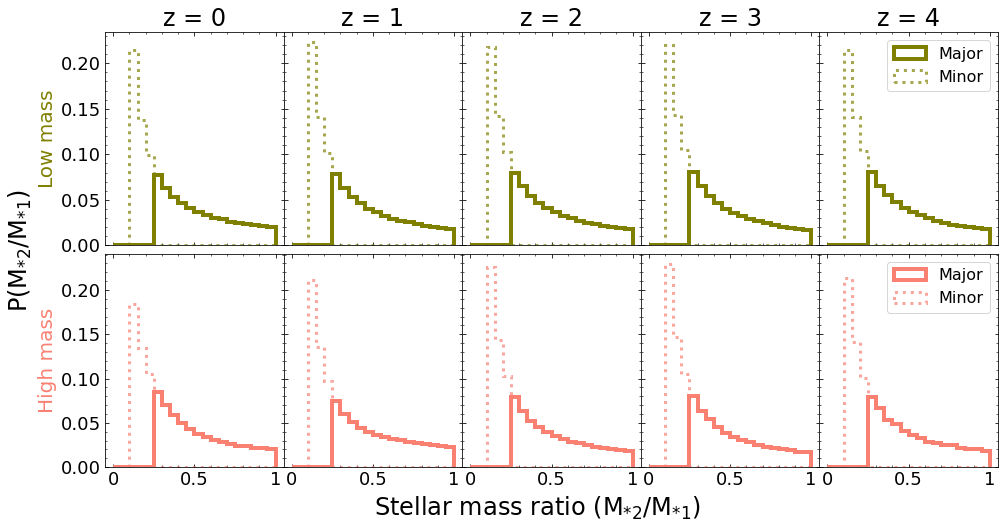
\includegraphics[width=\textwidth]{smrdist_1000.png}
    \caption{Stellar mass ratio distribution of all low mass (top) and high mass (bottom) pairs for all 1000 stellar mass realizations combined. Major pairs (solid lines) are defined as pairs with mass ratio $\ms{2}/\ms{1} > 1/4$, while minor pairs (dotted lines) are defined as pairs with stellar mass ratio $1/10<\ms{2}/\ms{1}<1/4$. Overall, the stellar mass ratio distribution of major and minor pairs of low and high mass galaxies show little evolution from $z=4$ (right) to $z=0$ (left). 
    Major pairs make up $51-55\%$ of the full sample of pairs at every redshift for both low and high mass pairs.}
    \label{fig:massratio}
\end{figure*}
% end pair prop plots %  
%%%%%%%%%%%%%%%%%%%%%%%

%%%%%%%%%%%%%%%%%%%%
% Pair prop. start %
\section{Sample: Overview of pair properties} \label{sec:pairprops}
    Utilizing the \paircat, for each snapshot, we compute the total number of primaries (isolated and paired) and pairs in each of the 1000 realizations, then take the median and 1 and 99 percentile spread on the median over all realizations. 
    Additionally, we compute the low and high mass total pair fraction (the total number of pairs, $\rm N_{pair}$, divided by the total number of primaries $\rm N_{prim}$) for each individual realization, then find the median and spread over all 1000 realizations. 
    
    Fig.~\ref{fig:counts} shows the median number (solid and dashed lines) of identified low and high mass primaries and pairs over the redshift range $z=0-4$.   
    The shaded regions show the 1-99\% spread of the set, though the spread is hard to distinguish in the low mass case.
    
    The number of identified primaries is lowest at $z=4$, and rises to a maximum around $z=1$ for both low and high mass primaries.
    The median count of low mass primaries (green solid line in top left panel) reaches a maximum of $\sim15000$ halos at $z\sim0.6$, then decreases by $\sim16\%$ to 12000 halos at $z=0$. 
    The count of high mass primaries (pink solid line in top right panel) reaches a maximum of $\sim2000$ at $z\sim1$, then remains approximately constant to $z=0$. 
    There are roughly 8 times as many low mass primaries as high mass primaries. 

    Unlike the primary count, the pair counts for low and high mass pairs peak at very different redshifts. 
    The count of low mass pairs (green dashed line) peaks much earlier at $z\sim2$ with $\sim3000$ pairs, and decreases to $\sim1000$ pairs at $z=0$.
    % From $z=4$ to $z=2$, the number of dwarf primaries doubles, as does the number of pairs due to the growth of structures over cosmic time.
    The pair count for high mass galaxies (pink dashed line), on the other hand, behaves more similarly to the primary count, increasing from $z=4$ to a peak at $z\sim1$, then leveling off through $z=0$. 

    The bottom panel of Fig.~\ref{fig:counts} shows the total pair fraction for low mass and high mass pairs, or equivalently, the fraction of primaries with a companion.
    The total pair fractions for both low and high mass pairs are roughly flat for $z=2.5-4$, and display opposite behavior for low redshifts between $z=0-2.5$. 
    The low mass pair fraction decreases from $\sim0.24$ to $\sim0.08$, a decrease of roughly $65\%$, while the high mass pair fraction remains flat between $z=1-2.5$.
    At very low redshifts, from $z=0-0.25$, the high mass pair fraction spikes sharply from $\sim 0.29$ to $\sim 0.36$, an increase of $25\%$.

    In Fig.~\ref{fig:massratio}, we show the combined distribution of stellar mass ratios of every pair from all 1000 realizations in the \paircat.
    Major pairs make up $51-55\%$ of the full sample of pairs at every redshift for both low and high mass pairs.
    In general, the shape of the distribution remains constant from $z=0$ (left) to $z=4$ (right) for both low and high mass pairs, and is thus independent of mass scale and of redshift. 

%%%%%%%%%%%%%%%%%%%%%%%%%
%%%%%%%%%%%%%%%%%%%%%%%%%
% Begin Results section %

\section{Results: The frequency of low mass and high mass pairs}
We have created catalogs of isolated low and high mass galaxy pairs from $z=0-4$ in the TNG100 simulation. 
In this section, we will analyze the occurrence rate of major and minor pair types across cosmic time. 

We are interested in the aggregate properties of the full sample, and so we will treat each stellar mass realization in the \paircat\ as an independent sample. 
At each snapshot, we calculate the median occurrence rate of each of the 1000 realizations. 
From this set of 1000 medians, we calculate the median and percentile spread which is shown in the following plots at the solid or dashed line, and the shaded region, respectively. 

In Sec.~\ref{sec:results-frac}, we show the redshift evolution of the fraction of primaries with a major or minor companion (the ``pair fraction") and compare the results for low mass and high mass pairs.
In Sec.~\ref{sec:results-frac-sepcut}, we look at the redshift evolution of pair fraction as a function of pair separation. 
% In Sec.~\ref{sec:results-scaled}, we compare the separations and velocities scaled by the FoF group's virial properties. 
% Finally, in Sec.~\ref{sec:results-virialcut}, we take subsets of the Pair Catalog, selecting only pairs within some fraction of the virial radius, and illustrate the impact on the recovered low and high mass pair fractions. 


%%%%%%%%%%%%%%%%%%%%%%%%%
% Pair fraction section %
    \subsection{Major and minor pair fractions}\label{sec:results-frac}
    We determine the occurrence rate of a major or minor pair by calculating the pair fraction. 
    The pair fraction is defined here as the ratio of the number of pairs to the total number of isolated \textit{and} paired primaries:
    $$f_{p}=\rm \frac{N_{pairs}}{N_{primaries}}.$$
    For example, the pair fraction of low mass major pairs is the number of low mass major pairs divided by the number of low mass primaries. 
    The pair fraction can be understood as a measure of the likelihood of finding a companion of a certain mass type about a primary identified in the field.
    
    Fig.~\ref{fig:pairfrac} shows the pair fractions calculated for low and high mass pairs (including both major and minor pairs separately) as a function of time for $z=0-4$. 
        % differences between major and minor pairs? 
    The pair fraction of minor pairs is less than that of major pairs for both low and high mass pairs at all redshifts, due to the lower stellar mass ratio limit we put on our pairs.
    If we lower the stellar mass ratio floor for minor pairs, the minor pairs would outnumber the major pairs.
    % Expanding the mass ratio criteria of our minor pair sample to include stellar mass ratios between 1/10-1/100 in our minor pair sample increases the fraction of minor pairs by a factor of $>2$ for massive pairs and between $~1.5-2x$ for dwarf pairs. \kc{are there any additional takeaways from this? }
    
        % differences between massive and dwarf pairs? 
    The low mass pair fraction evolves distinctly from that of high mass pairs.
    Low mass major and minor pair fractions start at their minima at $z=0$, and increase by about 200\% by $z\sim2-2.5$, at which point they level off and remain constant from $z=3-4$. 
    On the other hand, high mass pair fractions reach their maxima at $z=0$, then abruptly declining to $z\sim0.25$, before remaining approximately constant from $z=1-4$. 
    
        % difference panels
    The bottom panels of Fig.~\ref{fig:pairfrac} shows the low mass pair fraction subtracted from the high mass pair fraction (labelled ``$\rm High-Low$").
    The pair fraction difference reaches a maximum at $z=0$ for both major and minor pairs, and declines to $z\sim2-2.5$. 
    From $z=2.5-4$, the difference is approximately 0, and thus both major and minor pairs of high and low mass are equivalently common. 
    
        % takeaways 
    Overall, these results show that low mass and high mass pair counts evolve differently over time, particularly at very low redshift, despite the pair fractions being roughly equal at higher redshift. 
    The implications for the difference in the evolution of pair fractions for low mass and high mass pairs across time is discussed in detail in Sec.~\ref{sec:discussion}.
    
        % pair fraction plot
    \label{sec:results}
    \begin{figure*}[htp]
      \centering
      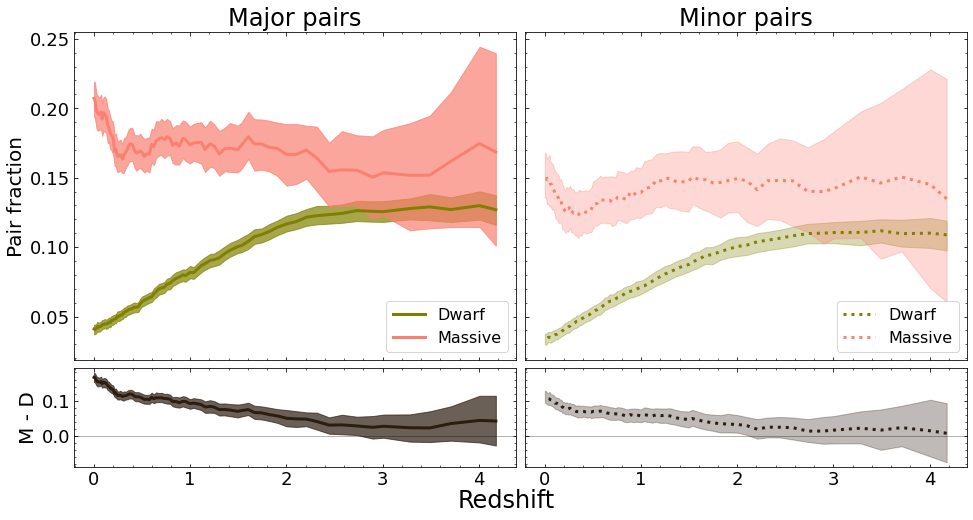
\includegraphics[width=\textwidth]{pairfrac_1000.png}
      \caption{% Top plots ~
        (Top) Median pair fraction, defined as the fraction of low mass or high mass primaries with a major (solid) or minor (dashed) companion by stellar mass (see Sec.~\ref{sec:methods-pairs}). 
        Shaded areas show the 1-99 percentile range on the median (solid and dashed lines) from 1000 stellar mass realizations. 
          % massive pairs
        The high mass pair fraction (pink) remains approximately constant for $z>1$, for both major and minor pairs. 
        Between $z=0.3$ and $z=0$, the major pair fraction increases from $0.163^{+0.011}_{-0.010}$ to $0.207^{+0.012}_{-0.014}$, while the minor pair fraction increases from $0.125^{+0.017}_{-0.014}$ to $0.152^{+0.016}_{-0.017}$.
          % dwarf pairs
        Low mass pair fractions, shown in green, are approximately constant from $z=3-4$, then decline monotonically to $z=0$. The major pair fraction is $0.041^{+0.003}_{-0.004}$ at $z=0$ and $0.126^{+0.008}_{-0.007}$ at $z=3$, while the minor pair fractions are $0.034\pm0.004$ and $0.111\pm0.008$ at $z=0$ and $z=3$, respectively. 
        % Bottom plots ~
        (Bottom) The median subtracted difference between high and low mass pair fractions, with the shaded $1$-$99$ percentile range from 1000 abundance matching realizations. The pair fraction difference increases with decreasing redshift, peaking at $z=0$ with a difference of $0.166\pm0.013$ for major pairs and $0.111\pm0.017$ for minor pairs. This shows that the redshift evolution of the pair fractions of low and high mass pairs proceeds differently, particularly at low redshift.}
      \label{fig:pairfrac}
    \end{figure*}
% end pair fraction 
%%%%%%%%%%%%%%%%%%%%%%%%%

%%%%%%%%%%%%%%%%%%%%%%%%%%%%%
% begining separation cut-pair fraction results %

\subsection{Major pair fractions as a function of maximum separation}\label{sec:results-frac-cuts}
    We also analyze subsets of the low and high mass major pairs that pass additional separation criteria. 
    Here, we study two different sets of separation criteria to compare the resulting pair fractions of subsets of the low and high mass major pairs to the full sample shown in Fig.~\ref{fig:pairfrac}.
    The first separation criteria that we employ selects pairs of different separations as a function of the size of the group's halo, as discussed in Sec.~\ref{sec:results-frac-vircut}. 
    In Sec.~\ref{sec:results-frac-sepcut}, we use physical 3D separation cuts to compare the population of low separation major pairs of low and high mass. 

\subsubsection{Separation cut - fraction of the virial radius}\label{sec:results-frac-vircut}
    \todo{here! }
              Interestingly, the recovered fraction of the full sample at <0.5rvir is <50\% but still closely resembles the full pair frac at z<2! thus, at low z, the behavior of the pair fractions is dominated by halos within 0.5 Rvir ~~ 


    %figures
    %%%%%%%%%%%%%%%%%%%%
    \begin{figure*}[htp]
        \centering
        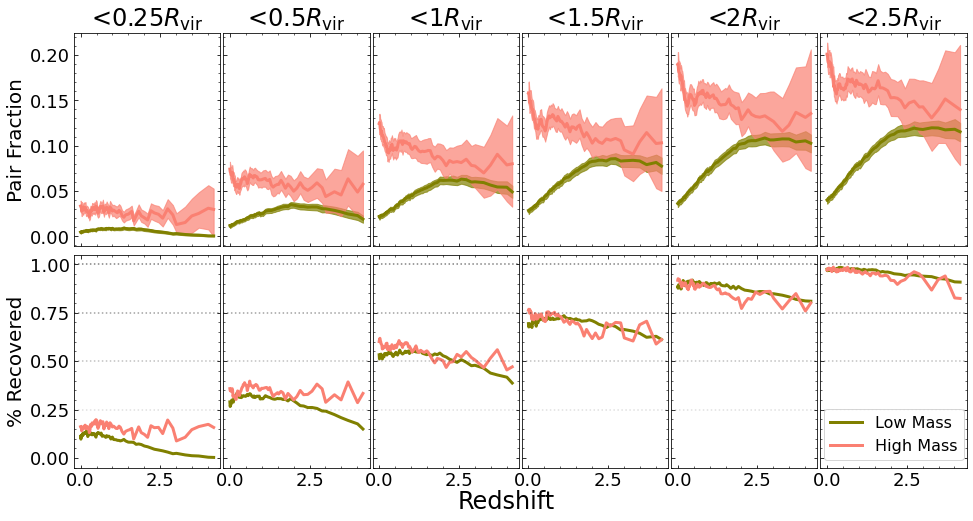
\includegraphics[width=\textwidth]{pairfrac_vircut.png}
        \caption{ The pair fraction of the subset of high mass (pink) and low mass (green) pairs with 3D separations within a fraction of the group's virial radius (see Sec.~\ref{sec:results-frac-sepcut} for details of calculations). 
        The median and 1-99 percentile spread are shown by the solid lines and shaded regions, respectively.
        Pair fractions for the subsample of low and high mass pairs with separations less that 0.25\Rvir are constant or declining with increasing redshift, and do not resemble the pair fractions for the full pair sample. 
        However, increasing the maximum separation of a pair to $0.5\Rvir$ leads to low and high mass major pair fractions that take on the same behavior as the full sample for $z<2$, where the low mass pair fraction decreases, and the high mass pair fraction (on average) increases. 
        The pair fraction trends for the low and high mass subsamples become similar to those of the true pair fractions (as seen in Fig.~\ref{fig:pairfrac}) when all pairs within $1.5\Rvir$ are included in the subsample.
      % bottom plot
        (Bottom) The fraction of the total collection of pairs in the subset of pairs that passes each separation cut.
        More than 50\% of low and high mass pairs have separations $<1.5\Rvir$ at all redshifts. 
        When the maximum separation is increased to $2.5\Rvir$, the recovery rate at all redshifts is $>90\%$ for low mass pairs, and $>80\%$ for high mass pairs. 
        }
      \label{fig:vircut}
    \end{figure*}
    %%%%%%%%%%%%%%%%%%%%

\subsubsection{Separation cut - physical separations}\label{sec:results-frac-sepcut}
    We calculate the pair fraction for all major low mass and high mass pairs, excluding pairs that exceed separations of $(50,70,100,150,200,300)\kpc$. 
    This additional separation criterion creates subsamples of the \paircat, and contains low and high mass pairs with separations between $15-50\kpc$, $15-70\kpc$, and so on\footnote{See Sec.~\ref{sec:methods-pairs} for a description of the $15\kpc$ lower separation cutoff.}.

    Fig.~\ref{fig:sepcut} shows the pair fractions for the subsamples of pairs with separations lower than the physical separation listed at the top of each column. 
    Similarly to the previous pair fraction plots, the top row presents the total median (solid line) of the collection of 1000 individual medians from each realization, and the shaded regions show the 1-99\%ile spread on the same collection of individual medians. 
    The bottom row of the plot shows the "recovery fraction", or the number of pairs in each subsample compared to the full sample of major pairs.
    
    As the maximum separation increases (left to right), so too does the pair fraction, as you begin to include more and more of the distantly separated pairs, as well as the recovery fraction. 
    The low mass major pair fraction (green) maintains roughly the same behavior (decreasing with decreasing redshift) for each separation cut, and closely resembles the pair fraction of the full sample (in Fig.~\ref{fig:pairfrac}) for maximum separation cuts higher than $150\kpc$. 
    The low mass pair fraction does not change significantly by excluding pairs with separations $>150\kpc$, thus the pair fraction profile is dominated by the closest 50\% of low mass pairs. 

    On the other hand, none of the subsamples of the high mass pairs display similar behavior to the full sample. 
    In particular, for smaller separation cuts (50\kpc or 70\kpc), the redshift evolution of the pair fraction more closely resembles the low mass pairs.
    For $r_{sep}<300\kpc$, the trends in the high mass major pair fraction is only similar at $z>1.5$, where it levels off, rather than continues to increase at higher $z$. 

    The recovery rate for low mass pairs is universally higher than for high mass pairs.
    By increasing the allowed separations $300\kpc$, virtually all low mass pairs are included in the subsample, with $>90\%$ of the total sample at $z=0$, and $\sim100\%$ for $z>1$.
    However, high mass pairs have a median separation of $\sim300\kpc$ at $z=0$, which means the recovery rate for low separation high mass pairs is very low. 
    In order to get a recovery fraction of at least 50\% at all redshifts from $z=0-4$, the subset of high mass pairs must include pairs with separations at least up to $300\kpc$.
    
    %figures
    %%%%%%%%%%%%%%%%%%%%
    \begin{figure*}[htp]
        \centering
        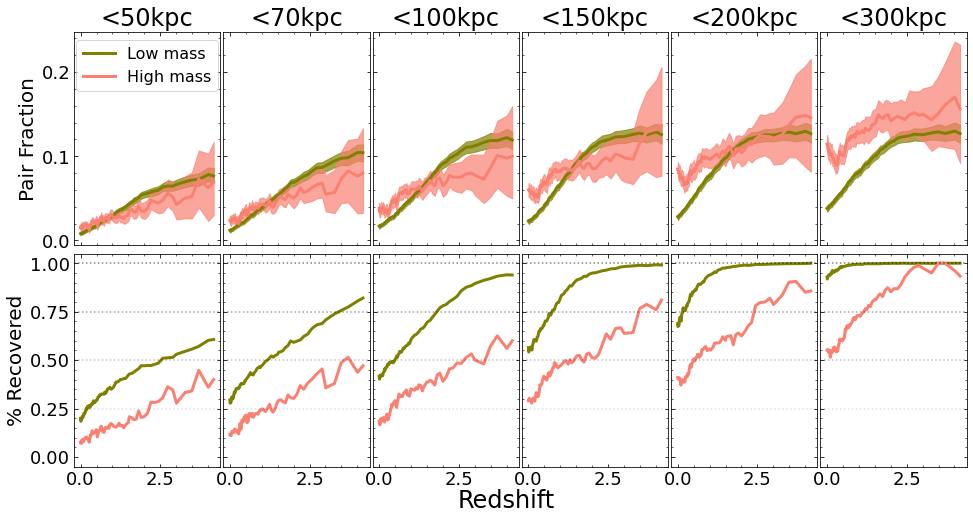
\includegraphics[width=\textwidth]{pairfrac_sepcut.png}
        \caption{      % top plot
        (Top) The major pair fraction of the subset of high mass (pink) and low mass (green) pairs with 3D separations less than the value given at the top of each column. 
        The median and 1-99 percentile spread are shown by the solid lines and shaded regions, respectively. 
        % what do we notice
        The behavior of the redshift evolution of major pair fractions for low and high mass pairs is strongly dependent on the maximum separation included in the subset.
        Pair fractions of low mass and high mass pairs are nearly indistinguishable for the lowest separation pairs $r_{sep}<50\kpc$ at every redshift. 
        For $z<2$, the true pair fraction behaviour (as seen in Fig.~\ref{fig:pairfrac}) becomes distinguishable when the maximum separation is $300\kpc$.
      % bottom plot
        (Bottom) The fraction of the total collection of pairs in the subset of pairs that passes each separation cut.
        Less than 50\% of massive pairs have separations $r_{sep}<50\kpc$, and 50-100\% have separations $r_{sep}<300\kpc$. 
        Between 20-60\% of low mass pairs have separations $r_{sep}<50\kpc$, while a separation cut of $r_{sep}<300\kpc$ captures roughly 100\% of the low mass pair population at all redshifts. 
        }
      \label{fig:sepcut}
    \end{figure*}
    %%%%%%%%%%%%%%%%%%%%
% end Results section%
%%%%%%%%%%%%%%%%%%%%%%


%%%%%%%%%%%%%%%%%%%%%%%%%%%%
% Begin Discussion section %
\section{Discussion}\label{sec:discussion}

% In particular, we study dwarf galaxy pairs and massive galaxy pairs that are of similar stellar and halo mass to a variety of galaxy pairs in the Local Group. 
% We categorize these pairs into one of four pair types: massive major pairs, such as the MW+M31; massive minor pairs, such as M31+M33 or MW+LMC; dwarf major pairs, such as M33+LMC; and finally, dwarf minor pairs, such as the LMC+SMC.
% \kc{can maybe move these two sentences to a discussion section}
    
%     \kc{ make a subsection about the equivalence of our findings with the dark matter simulation) We make brief note of results for our equivalent analysis using the dark matter only TNG100-Dark simulation as well in Sec.~\ref{sec:results}.}

% \subsection{Implications for the differences in pair fractions of dwarf and massive pairs}
% In Sec.~\ref{sec:results-frac}, we presented the pair fraction of massive and dwarf galaxy pairs and found that the relative frequency of the two populations evolve distinctly from $z=0-4$. 
% While the frequency of massive pairs compared to the number of massive primaries is roughly constant and become more common at low redshift, dwarf major and minor pairs become more than 50\% less common at $z=0$ compared to $z=2$. 
% Since scaled separations and velocities do not change drastically between dwarf and massive pairs, the difference in the evolution of the pair fractions indicates that the merger processes of each population may proceed differently.

% % One scenario that could explain this behavior is a very rapid merger timescale for dwarf pairs, and a slower merger timescale for massive pairs. 
% % In this case, dwarf pairs will merge quickly after formation, thus depleting the number of dwarf pairs at later times. 
% % Simultaneously, the merged remnant of a dwarf pair is likely to join the population of isolated primaries until star formation finally pushes the stellar mass up into the massive primary regime.
% % The likelihood of a dwarf pair becoming a massive primary with a minor companion is very small, since only XX\% of dwarf pairs have a major tertiary companion. \kc{calculate the number of }

% % Alternatively, if the dark matter halo and stellar mass of a dwarf galaxy pair increase enough through cosmic accretion or very minor mergers from $z=4$ to $z=2$, the pair will be reclassified as a massive pair at later times. 

% For example, dwarf galaxy merger timescales may be significantly shorter than massive galaxy merger timescales, which would deplete the population of dwarf galaxy pairs by low redshift. 
% Additionally, early dwarf galaxy mergers may result in systems that are identified as massive pairs at late times, and massive pairs may grow such that they exceed our mass criteria, thus leading to an apparent overall decrease in the number of pairs. 
% The drop in the absolute number of dwarf and massive primaries at low z as shown in Fig.~\ref{fig:counts} indicates that indeed many of these systems leave the mass range specified by our selection criteria between $z=0-1$. 
% However, since the number of dwarf primaries is roughly constant between $z=0.5-1.5$, but the number of pairs is still decreasing during this time, this indicates that mergers are occurring during this time, and not yet leaving the mass regime specified. 
% In fact, the number of dwarf pairs that are removed from the sample from $z=0$ to $z=2$ is 10 times greater than the total number of massive pairs, indicating that these pairs are not simply accreting matter and moving into the higher mass bin.





% \subsection{Comparison to previous pair fraction studies}
% We performed a pair fraction analysis for dwarf and massive galaxy pairs in the TNG100 simulation, utilizing the full 6D position and velocity information that simulations enable. 
% However this means that direct comparison to pair fractions reported from observations is not straight-forward, as observationally selected pairs uniquely suffer from contamination, due to projected pairs, and restrictive separation criteria, that exclude more widely separated pairs. 
% Fortunately, a number of previous studies of pair fractions in the Illustris simulations have used lightcones to create mock images of observationally-motivated fields, from which they select pairs in the same fashion that is typically done with observational data.
% These studies select simulated galaxies based on stellar mass, and then use cuts on the projected separation and line of sight velocity difference to select pairs, which permits direct comparison between simulations and observations. 

% At the low mass end, \citet{Besla2018} quantified dwarf galaxy pair fractions in Illustris-1, both projected and 3D pairs, which enabled a direct comparison of the cosmologically-derived pair fractions with an equivalently selected dwarf pair fraction from SDSS.  
% The pair selection criteria for dwarf galaxies, here defined as stellar masses\footnote{The stellar masses of galaxies from the Illustris simulations used in \citet{Besla2018} are from the median of the \citet{Moster2013} abundance matching prescription, the same as used in this work, rather than the stellar mass values from the simulations.} from $2\times10^{8} < M_{*} < 5\times10^{9}\,\Msun$, include a projected separation criteria of $r_{p} < 150\,\kpc$ and a relative line-of-sight velocity difference $\Delta v_{\rm los} < 150\,\kms$. 

% By searching for pairs in a projected space while having access to the true 3D positions and velocities of the galaxies, they quantified the contamination fraction and found that up to $\sim40$\% of identified companions were unrelated but appeared to be close due to projection effects. 
% In Illustris, they found that the projected major pair fraction of dwarf galaxies at $z\sim0$ is $f_{p,proj.}\sim0.005-0.012$, while the . \kc{where tf are these numbers from??? }
% The total pair fraction (including all stellar mass ratios) is $0.032\pm0.005$ for the projected mock catalogs, which are consistent with SDSS equivalently-selected pairs, which find a total pair fraction of $0.035\pm0.3$. 

% However, using the full physical catalogs, they find a lower pair fraction of $0.02\pm0.004$. \kc{I *THINK* this is the fraction of TOTAL pairs (N\_1 from the tables)? not just major pairs? otherwise I don't know how it's different.}
% For comparison, when we modify our pair selection criteria to match those of \citet{Besla2018}, and require a 3D separation $r_{\rm sep}< 150\,\kms$ and a 3D relative velocity $\Delta v_{\rm los} < 150\,\kms$, we find a dwarf major pair fraction of XX at $z=0$, which is slightly SKZ than the \citet{Besla2018} results.
% This is/is not surprising because SKZ. 

% As the behavior of the major pair fraction as a function of primary stellar mass is consistent between the projected mock catalogs and the SDSS catalogs, they conclude that cosmological simulations can be used to reliably constrain observational pair fractions of dwarf mergers across time. \kc{across time... is this true?} 
% Additionally, which projected and 3D pair catalogs yield different absolute values of pair fractions, their behavioral trends as a function of mass are nearly identical such that, in terms of trends, projected and 3D pair fractions will yield similar results. 


% % While the study uses projected separations and line of sight velocities, we can assume that the same \textit{trends} are valid for full-6D selected pairs, such that our pair fraction trends can be reasonably compared to those in observations. 

% Separate studies have analyzed the pair fractions of higher mass galaxies in Illustris simulation. 
% In particular, \citet{snyder2017} created mock catalogs using lightcones in the Illustris-1 simulation to pick pairs in the same fashion as done in observations. 
% Specifically, they consider only major pairs with: $1\times 10^{11}>M_{*,1} >1\times 10^{10.5}Msun$, projected distances between $14\kpc-71\kpc$, and a redshift separation of $\Delta z<0.02(1+z_{pri}$, which corresponds to a velocity separation of $<1.8\time10^4\kms$. 
% They find that the major pair fraction for primaries with stellar mass $1\times 10^{10.5-11}Msun$ is constant or decreasing for $z>1$. 
% Additionally, they compared to observational studies \kc{what studies} that selected pairs with stellar mass $(M* > 10^{10.8}\Msun)$, $(10 <d/(kpc h-1) < 30)$, and $(Msec/Mpri > 0.1)$, and found good agreement between the measured pair fractions as a function of redshift.
% Thus, projected pair fractions in the Illustris simulation are likely representative of those found in observations for massive galaxy pairs.

% \citet{snyder2023} extended this work to utilize the TNG simulation, and created mock images of extragalactic survey fields mimicking future planned surveys like JADES.
% From the mock images, they calculated the pair fraction for major pairs with projected separations between $5-70 \kpc$ and with redshift separations of $\Delta z< 0.02(1+z)$, and also found flat or decreasing major pair fractions. 
% This is in agreement with our work, as our major pair fraction for massive galaxies is approximately constant or decreasing with higher redshift for $z>1$. 
% While we cannot directly compare the values of the pair fractions themselves, as the projected and 3D pair separations will yield very different pair fractions as shown in \citet{Besla2018}, we can say that the behavioral trends are the same. 
% Pair fractions computed using 3D separations do not have to account for contamination due to projection effects, which would increase the inferred pair fraction, however our separation criteria is much less stringent, which would also increase the pair fraction. 

% % Alejandro's paper connection: studies are finding good agreement between simulations and TNG, as evidenced by this paper. They found that TNG simulated images well approximated the morphologies of galaxies in the KIDS survey, although they were a bit more compact and lumpy. But this means that there is precedent for using TNG in these kinds of comparisons. 

% % ? maybe to do: plot with comparison values 
% \subsection{Implications for observational pair selection criteria}
%     %figures
%     %%%%%%%%%%%%%%%%%%%%
%     \begin{figure*}[htp]
%       \centering
%       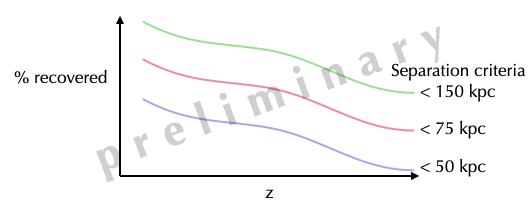
\includegraphics[width=\textwidth]{frac_selected.png}
%       \caption{ The fraction of total pairs selected with additional separation selection criteria as a function of redshift. 
%         }
%       \label{fig:frac-select}
%     \end{figure*}
%     %%%%%%%%%%%%%%%%%%%%

%     % outline
%     \begin{itemize}
%         \item examples of typical pair selection criteria (i.e. <75 kpc, velocity crit, etc.)
%         \item Show how low separation cuts affect pair fractions      
%         \item Sep distribution plot and explanation (text below) 
%         \item Plot of \% of total pairs selected as function of z for different separation criteria (or maybe better is to do total as function of separation, for different redshifts?) 
%         \item What does this mean for JWST and future surveys?
%     \end{itemize}
    
    
% % text on the separation distribution plot
% % Fig.~\ref{fig:sep-dist} shows the full distribution of separations for major and minor dwarf and massive pairs at $z=\{0,1,2,3,4\}$, and includes all 1000 AM realizations. 
% % For reference, the median at each corresponding redshift from Fig.~\ref{fig:sep} (that is, the median of the medians of each realization) are shown in light black vertical lines.
% % Each plot is normalized such that the area under an individual curve is 1.
%     % the redshift evolution
% % At $z=4$, all pair types (dwarf and massive, major and minor) have narrow distributions that pile up around 0 $\kpc$\footnote{Note that only pairs with separations $>10\kpc$ are included in this analysis, see Sec.~\ref{sec:methods-pairs}.}, with ranges between $10-150\,\kpc$ for dwarf pairs and $10-300\,\kpc$ for massive pairs. 
% % The distributions become more and more broad as $z\to0$, where separations range between $\sim10-400\,\kpc$ for dwarf pairs and $\sim10-1000\,\kpc$ for massive pairs.

% % Since the distribution of separations changes dramatically from $z=4$ to $z=0$, the population of low separation pairs that are selected at $z=4$ includes the majority of true pairs, but this is not the case at low z. 
% % At low z, separation criteria must be very broad to encompass the majority of pairs. 
% % Figure~\ref{fig:frac-select} shows the fraction of pairs that have separations less than $\{50, 75, 100, 150\}\kpc$.
% % At high redshift ($z\sim2-4$) a majority of pairs are included in the selection, however at lower redshift ($z\sim0-1$), the pair completeness decreases substantially, with fewer than XX\% of the total number pairs for XX separation criteria. 

% As JWST is expected to image dwarfs (give stellar mass range) out to z=XX in XX survey, the selection criteria for dwarf pairs that are applied will affect the inferred pair fractions greatly. 

% %%%%%%%%%%%%%%%%%%%%%%


% %%%%%%%%%%%%%%%%%%%%%%%%%%%%%%%%%%%
% \pagebreak

\section{Summary and Conclusions}\label{sec:summary}
% In this paper, we collect a large set of dwarf and massive subhalo pairs from the Illustris TNG100-1 simulation. 
% Pairs are selected from the full volume over all 100 snapshots of the simulation, though the sample size of pairs in the first 20 snapshots ($z>4.2$) is extremely small. 
% Major and minor pairs are determined using the stellar mass ratio between the primary and secondary halo using stellar masses from 1000 random realizations of the abundance matching prescription. 
% From this pair sample, we calculate the pair fractions and snapshot by snapshot kinematics of 4 different pair types: dwarf major pairs, dwarf minor pairs, massive major pairs, and massive minor pairs.

% Our main findings are as follows:
% \begin{itemize}
%     \item The pair fraction for dwarf and massive pairs does not proceed identically throughout cosmic time. In fact, the two mass scales have opposite behavior at low z. The number of dwarf pairs per dwarf primary decreases from $z=2\to0$, while the number of massive pairs per massive primary is approximately constant from $z=4\to0.25$, with an abrupt increase at lower redshift. 
%     \item The median 3D separation between the primary and secondary subhalo of a pair increases with decreasing redshift. The typical separation of a dwarf (massive) pair is $120\,\kpc$ ($240\,\kpc$) at $z=0$ and $40\,\kpc$ ($80\,\kpc$) at $z=4$.
%     \item The median relative velocity between the primary and secondary subhalo of a pair decreases towards lower redshift. The typical relative velocity of a dwarf (massive) pair is $70\,\kms$ ($175\,\kms$) at $z=0$ and $132\,\kms$ ($290\,\kms$) at $z=4$.
%     \item The separation scaled by the total virial radius of the group is similar for dwarf and massive pairs, though massive pairs tend to have lower scaled separations for redshifts between $z=0-2$. The relative velocity scaled by the circular velocity at the virial radius evolves identically for both dwarf and massive pairs, indicating that the relative velocities are self-similar at different mass scales. 
%     \item All of the above trends hold true for both major and minor pairs of the same mass range (i.e., the conclusions for the dwarf major pairs hold too for the dwarf minor pairs). 
% \end{itemize}

% Our results are consistent with prior works that have studied the pair fractions of massive and dwarf galaxies in the Illustris simulations in a projected sense. 
% The agreement between the pair fraction trends from projected and from 3D pair selection criteria points to the IllustrisTNG simulation's robust ability to reproduce the characteristics of galaxy pairs from observations. 

% Additionally, we conclude that:
% \begin{itemize}
%     \item Dwarf galaxy pairs and massive galaxy pairs likely have different evolutionary and merger processes which result in the opposing behavior of dwarf and massive pair fractions as a function of redshift.
%     \item The separation criteria used to observationally identify pairs likely results in an incompleteness of at least XX\% by $z=0$, though is less problematic for high redshift pairs where pairs tend to have smaller separations. 
% \end{itemize}

% Our conclusions point to the importance of time-evolving pair selection criteria that account for the natural separation increase of pairs at the universe expands. 


% \kc{other main takeaways?}

% \begin{itemize}
%     \item otherMain takeaways: (maybe include these within main findings bullets~)
%         \begin{itemize}
%             \item lit comp.
%             \item dwarfs not equal massives 
%             \item JWST imps.
%         \end{itemize}
%     \item Future work
% \end{itemize}

% Findings:
% \begin{itemize}
%     \item 
%     \item Median pair separations increase and relative velocities decrease from high to low redshift. 
% \end{itemize}

%%%%%%%%%%%%%%%%%%%%%%%%
%%%%%%%%%%%%%%%%%%%%%%%%

\bibliography{refs}{}
\bibliographystyle{aasjournal}

\end{document}
